\documentclass{beamer}

\usetheme{Antibes}
\usepackage{pgfplots}
\usepackage{graphicx}
\title{CONTROL SYSTEMS}
\subtitle{Presentation}
\author{Aashrith-EE18BTECH11035}


\begin{document}

\begin{frame}
\titlepage    
\end{frame}


\begin{frame}{EC GATE-2016 Q.NO-45 }
In the feedback system given below G(s)= \(\frac{1}{s^2+2s}\) .\\
The step response of the closed-loop system should have minimum settling time and have no overshoot.

\begin{figure}
    \includegraphics[scale=0.5]{figs/Presentation.png}
\end{figure}

The required value of gain k to achieve this is \underline{\hspace{2cm}}

\end{frame}

\begin{frame}{Solution}
$Settling Time$: The time required for the transient's damped oscillations to
reach and stay within ±2\% of the steady-state value.\vspace{5mm}


$Overshoot$:The amount that the waveform overshoots the steady state, or final, value at the peak time, expressed as a percentage of the steady-state
value.\\
\vspace{5mm}
The Transfer function of the negative unity feedback system is given by \(\frac{H(s)}{1+H(s)}\) (Where H(s) is the open-loop gain of the system) \\
\end{frame}
\begin{frame}
    

In the given Question H(s) = k x G(s).So, Transfer function of the whole feedback system is \(\frac{kG(s)}{1+kG(s)}\) \\
By Substituting G(s) function we get \(\frac{k}{s^2+2s+K}\)
\begin{figure}
    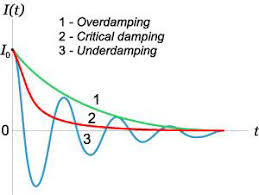
\includegraphics[scale=0.5]{figs/final1.jpeg}

    
\end{figure}

By observing the above figure,minimum settling time is obtained for Critical Damped System.\\
\end{frame}

\begin{frame}
Also, Critically Damped System doesn't have overshoot.\\
Transfer function of the Critical Damped System is given by
\(\frac{\omega_n^2}{s^2+2\zeta\omega_ns +\omega_n^2}\) (Where, \zeta=1)\\
By comparing Obtained Transfer function \(\frac{k}{s^2+2s+K}\) and the general transfer function of Critical Damped System \(\frac{\omega_n^2}{s^2+2\zeta\omega_ns +\omega_n^2}\)\\
\vspace{5mm}\\
We get \zeta = \(\frac{1}{\sqrt{K}}\)\\
As \zeta = 1\\
\vspace{5mm}\\
\(\frac{1}{\sqrt{K}}\) =1\\
\vspace{5mm}\\
K=1\\
\vspace{5mm}\\
Therefore, The value of K is 1.\\




\end{frame}
\begin{frame}
\title{Plot of the obtained Transfer Function}
\begin{figure}
    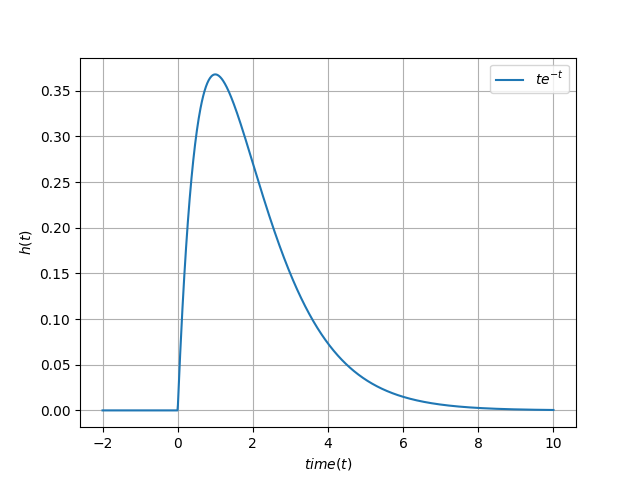
\includegraphics[scale=0.65]{figs/final.png}

    
\end{figure}



\end{frame}


\end{document}
